\chapter{Absence Of Information Is Also Knowledge}

This chapter presents an approach to the problem of learning object placement habits of humans in an occluded environment. Generally in domestic environments like our home, we humans prefer to store our food, cooking equipment, silverware and dishes inside closed cabinets like drawers, cupboards and refrigerators. This causes high level of occlusion for data collection.

We assume there is a domestic service robot which while interacting in human environments records all the information generated using vision sensor.
So for a domestic robot with only camera as a sensor, the chances of observing  these objects inside closed cabinets is drastically reduced.

\begin{figure}[htp]
\centering
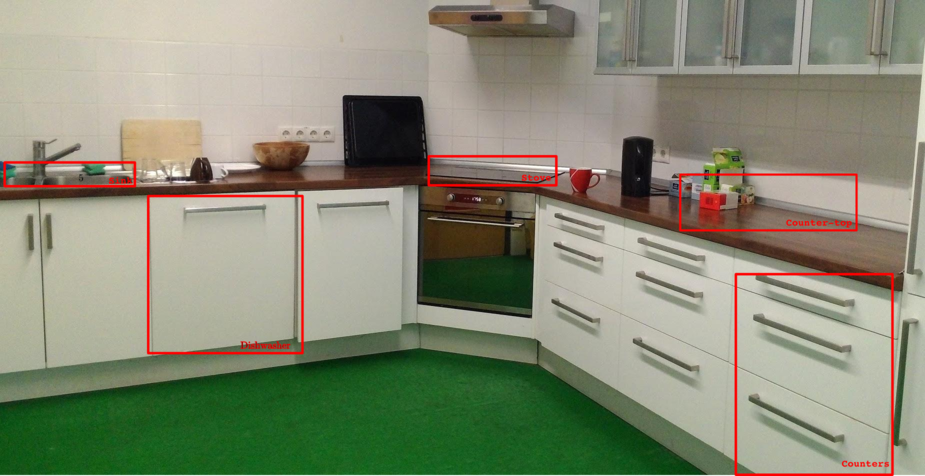
\includegraphics[width=0.8\textwidth]{images/kitchen_crop_ano.png}
\caption{Kitchen environment with occluded spaces}
\label{fig:kitchen occluded}
\end{figure}

The basic requirement of machine learning is data, from which information and knowledge can be learnt. But in highly occluded environments like kitchen its difficult for a domestic robot to make an observation of the object and record the object location.  Hence our hypothesis that we can learn knowledge about object locations quantitatively i.e. learning patterns from the data observed, becomes a herculean task to prove.

An alternative approach to counter the sparsity of data is by recording the absence of the object in visible locations and learning knowledge about where objects are not located. Consider an motivating example, as depicted in Figure \ref{fig:alllocations} . Here, a mobile robot is in a kitchen in the morning. The following locations can be scanned by the robot: kitchen-sink, counter-top and stove, while the cabinets, dishwasher and refrigerator are occluded. The robot will make observations of cup and kettle on counter-top , spoon on the sink top. Assume that the robot is also learning object locations of cooking pot. If the robot only records the observed objects then there is no data recorded for the cooking-pot and no knowledge is learned about the cooking-pot. \emph{A possible solution is to even record the \textbf{absence} of cooking-pot on the visible locations}. From this the robot can learn that the cooking-pot is less probable to be on the kitchen-sink, counter-top and stove during morning time. Supplementary the robot can also learn that there is higher probability for the cooking-pot being in the cabinet or dishwasher.

\begin{figure}
    \centering
    \begin{subfigure}[b]{0.3\textwidth}
        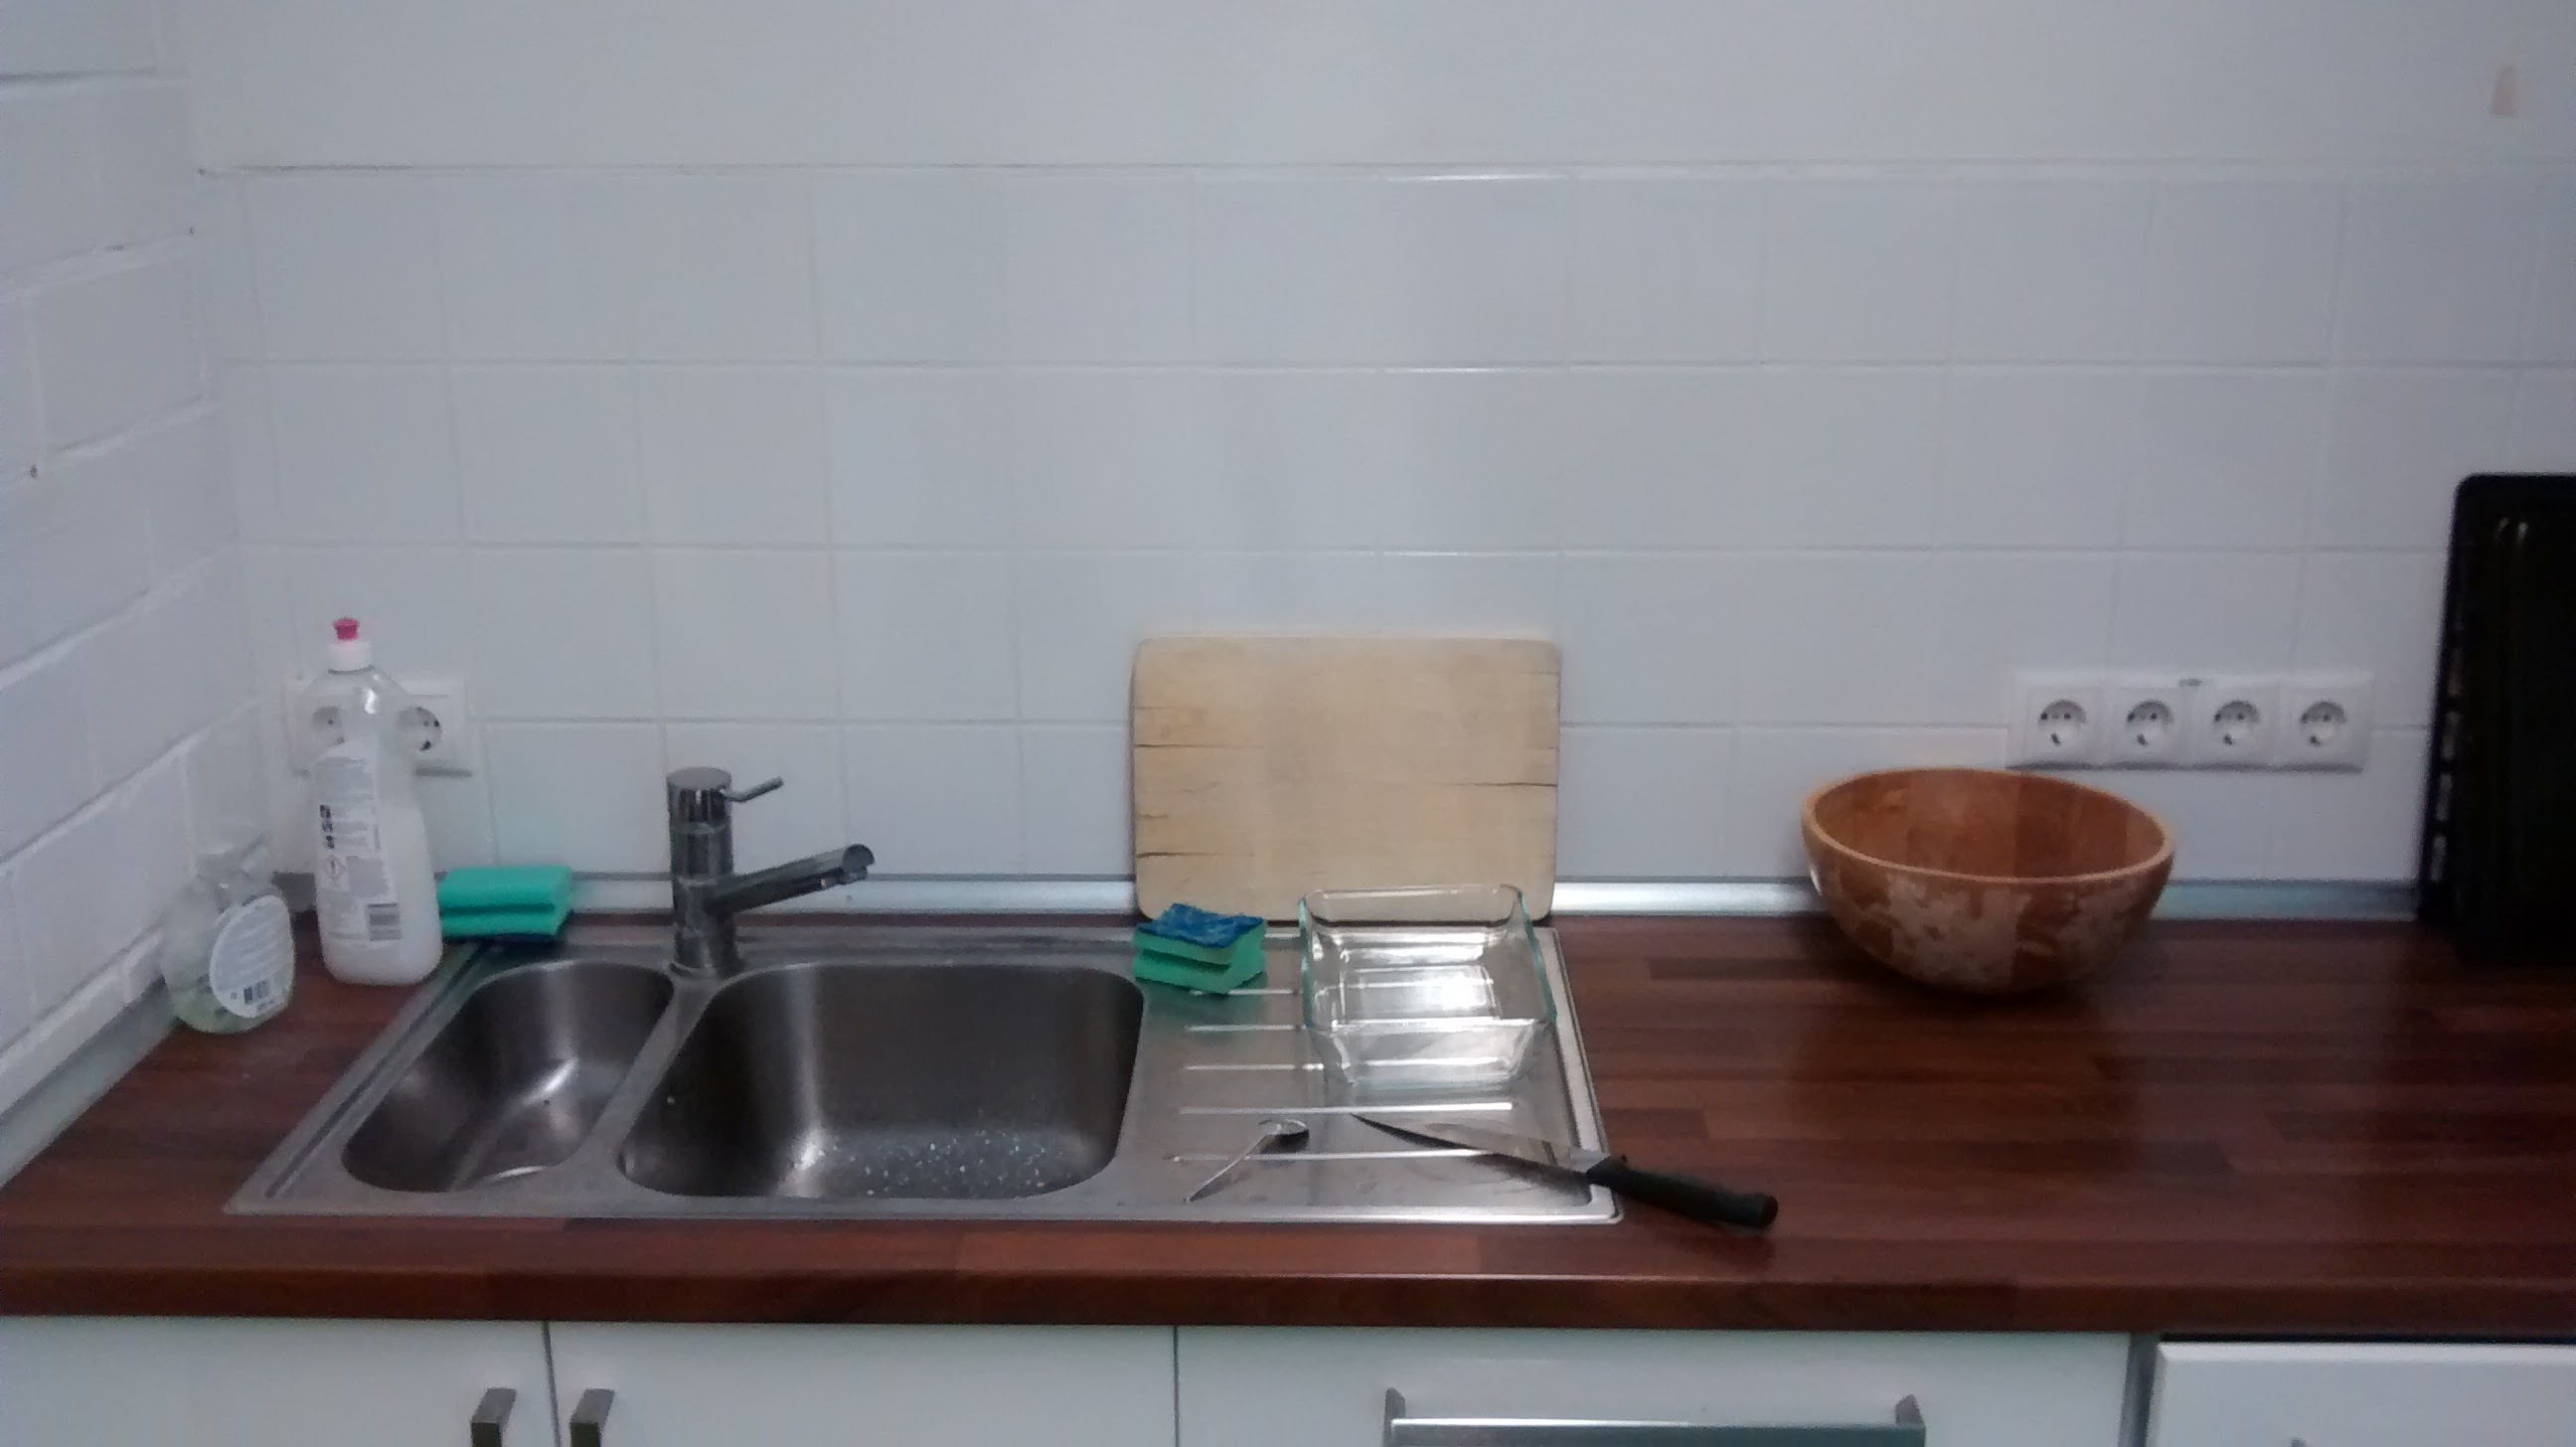
\includegraphics[width=\textwidth]{images/sink.jpg}
        \caption{Sink}
        \label{fig:sink}
    \end{subfigure}
    ~ %add desired spacing between images, e. g. ~, \quad, \qquad, \hfill etc. 
      %(or a blank line to force the subfigure onto a new line)
    \begin{subfigure}[b]{0.3\textwidth}
        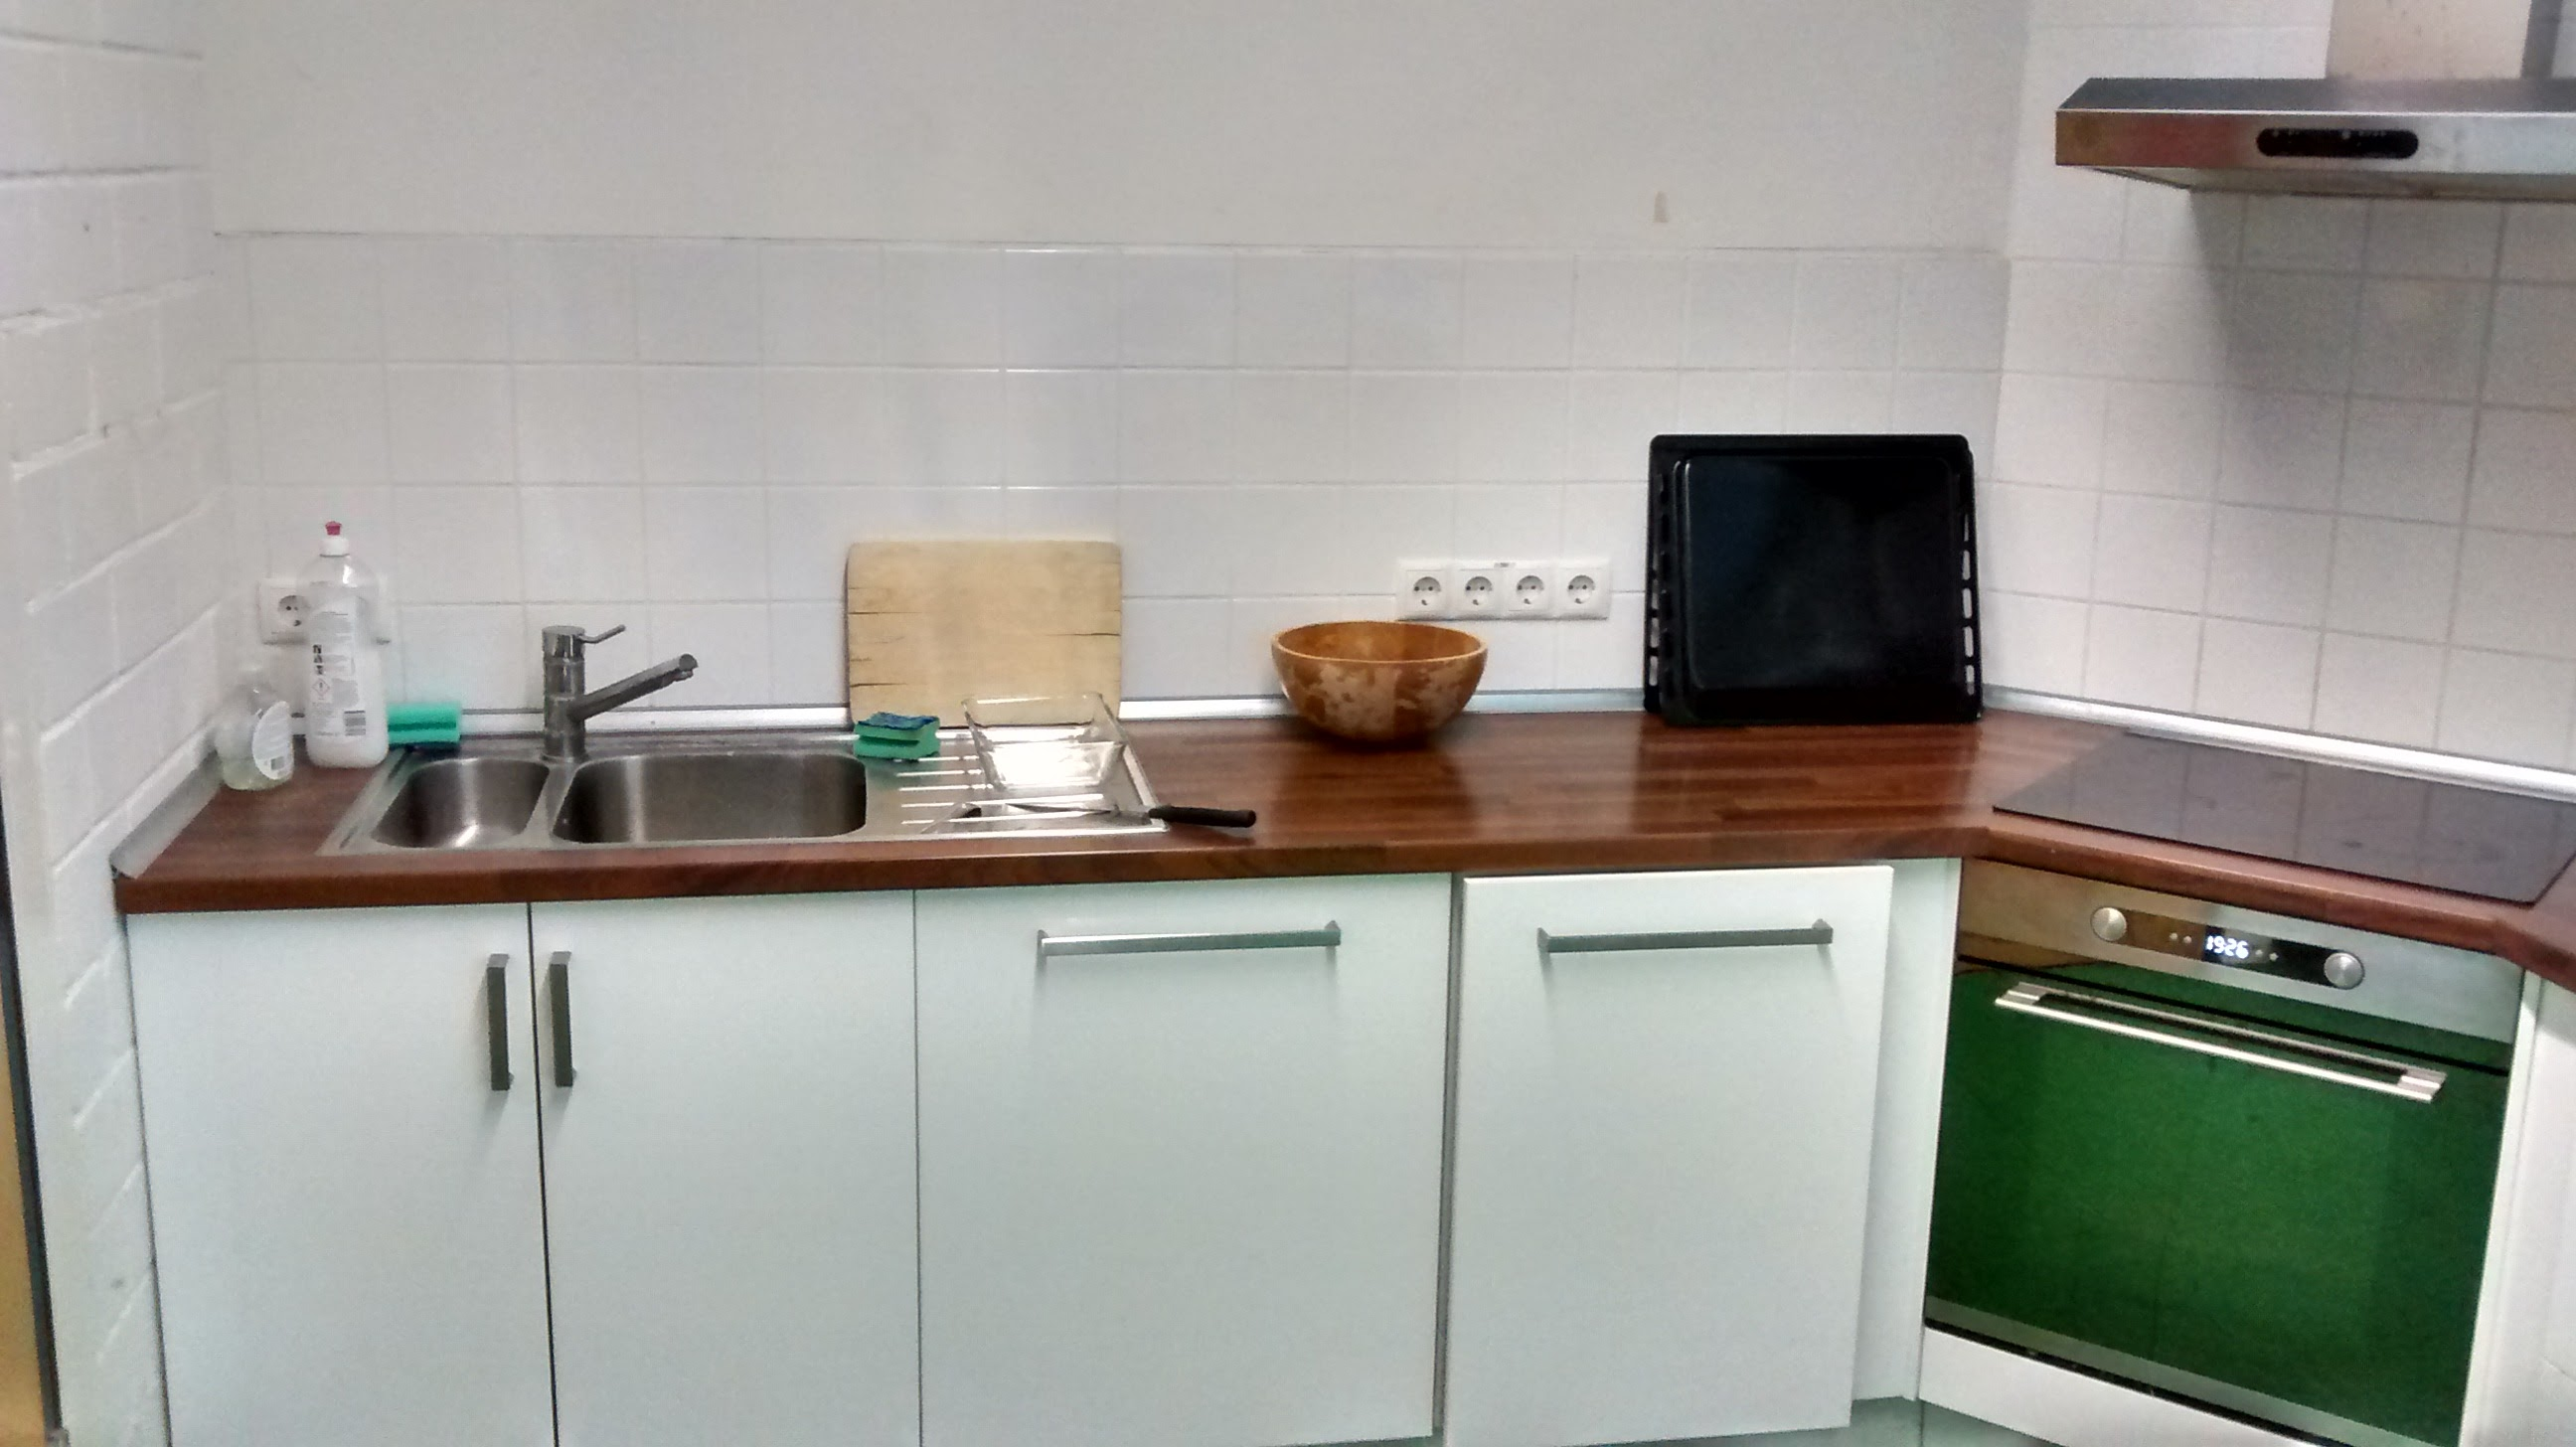
\includegraphics[width=\textwidth]{images/stove.jpg}
        \caption{Stove}
        \label{fig:stove}
    \end{subfigure}
    ~ %add desired spacing between images, e. g. ~, \quad, \qquad, \hfill etc. 
    %(or a blank line to force the subfigure onto a new line)
    \begin{subfigure}[b]{0.3\textwidth}
        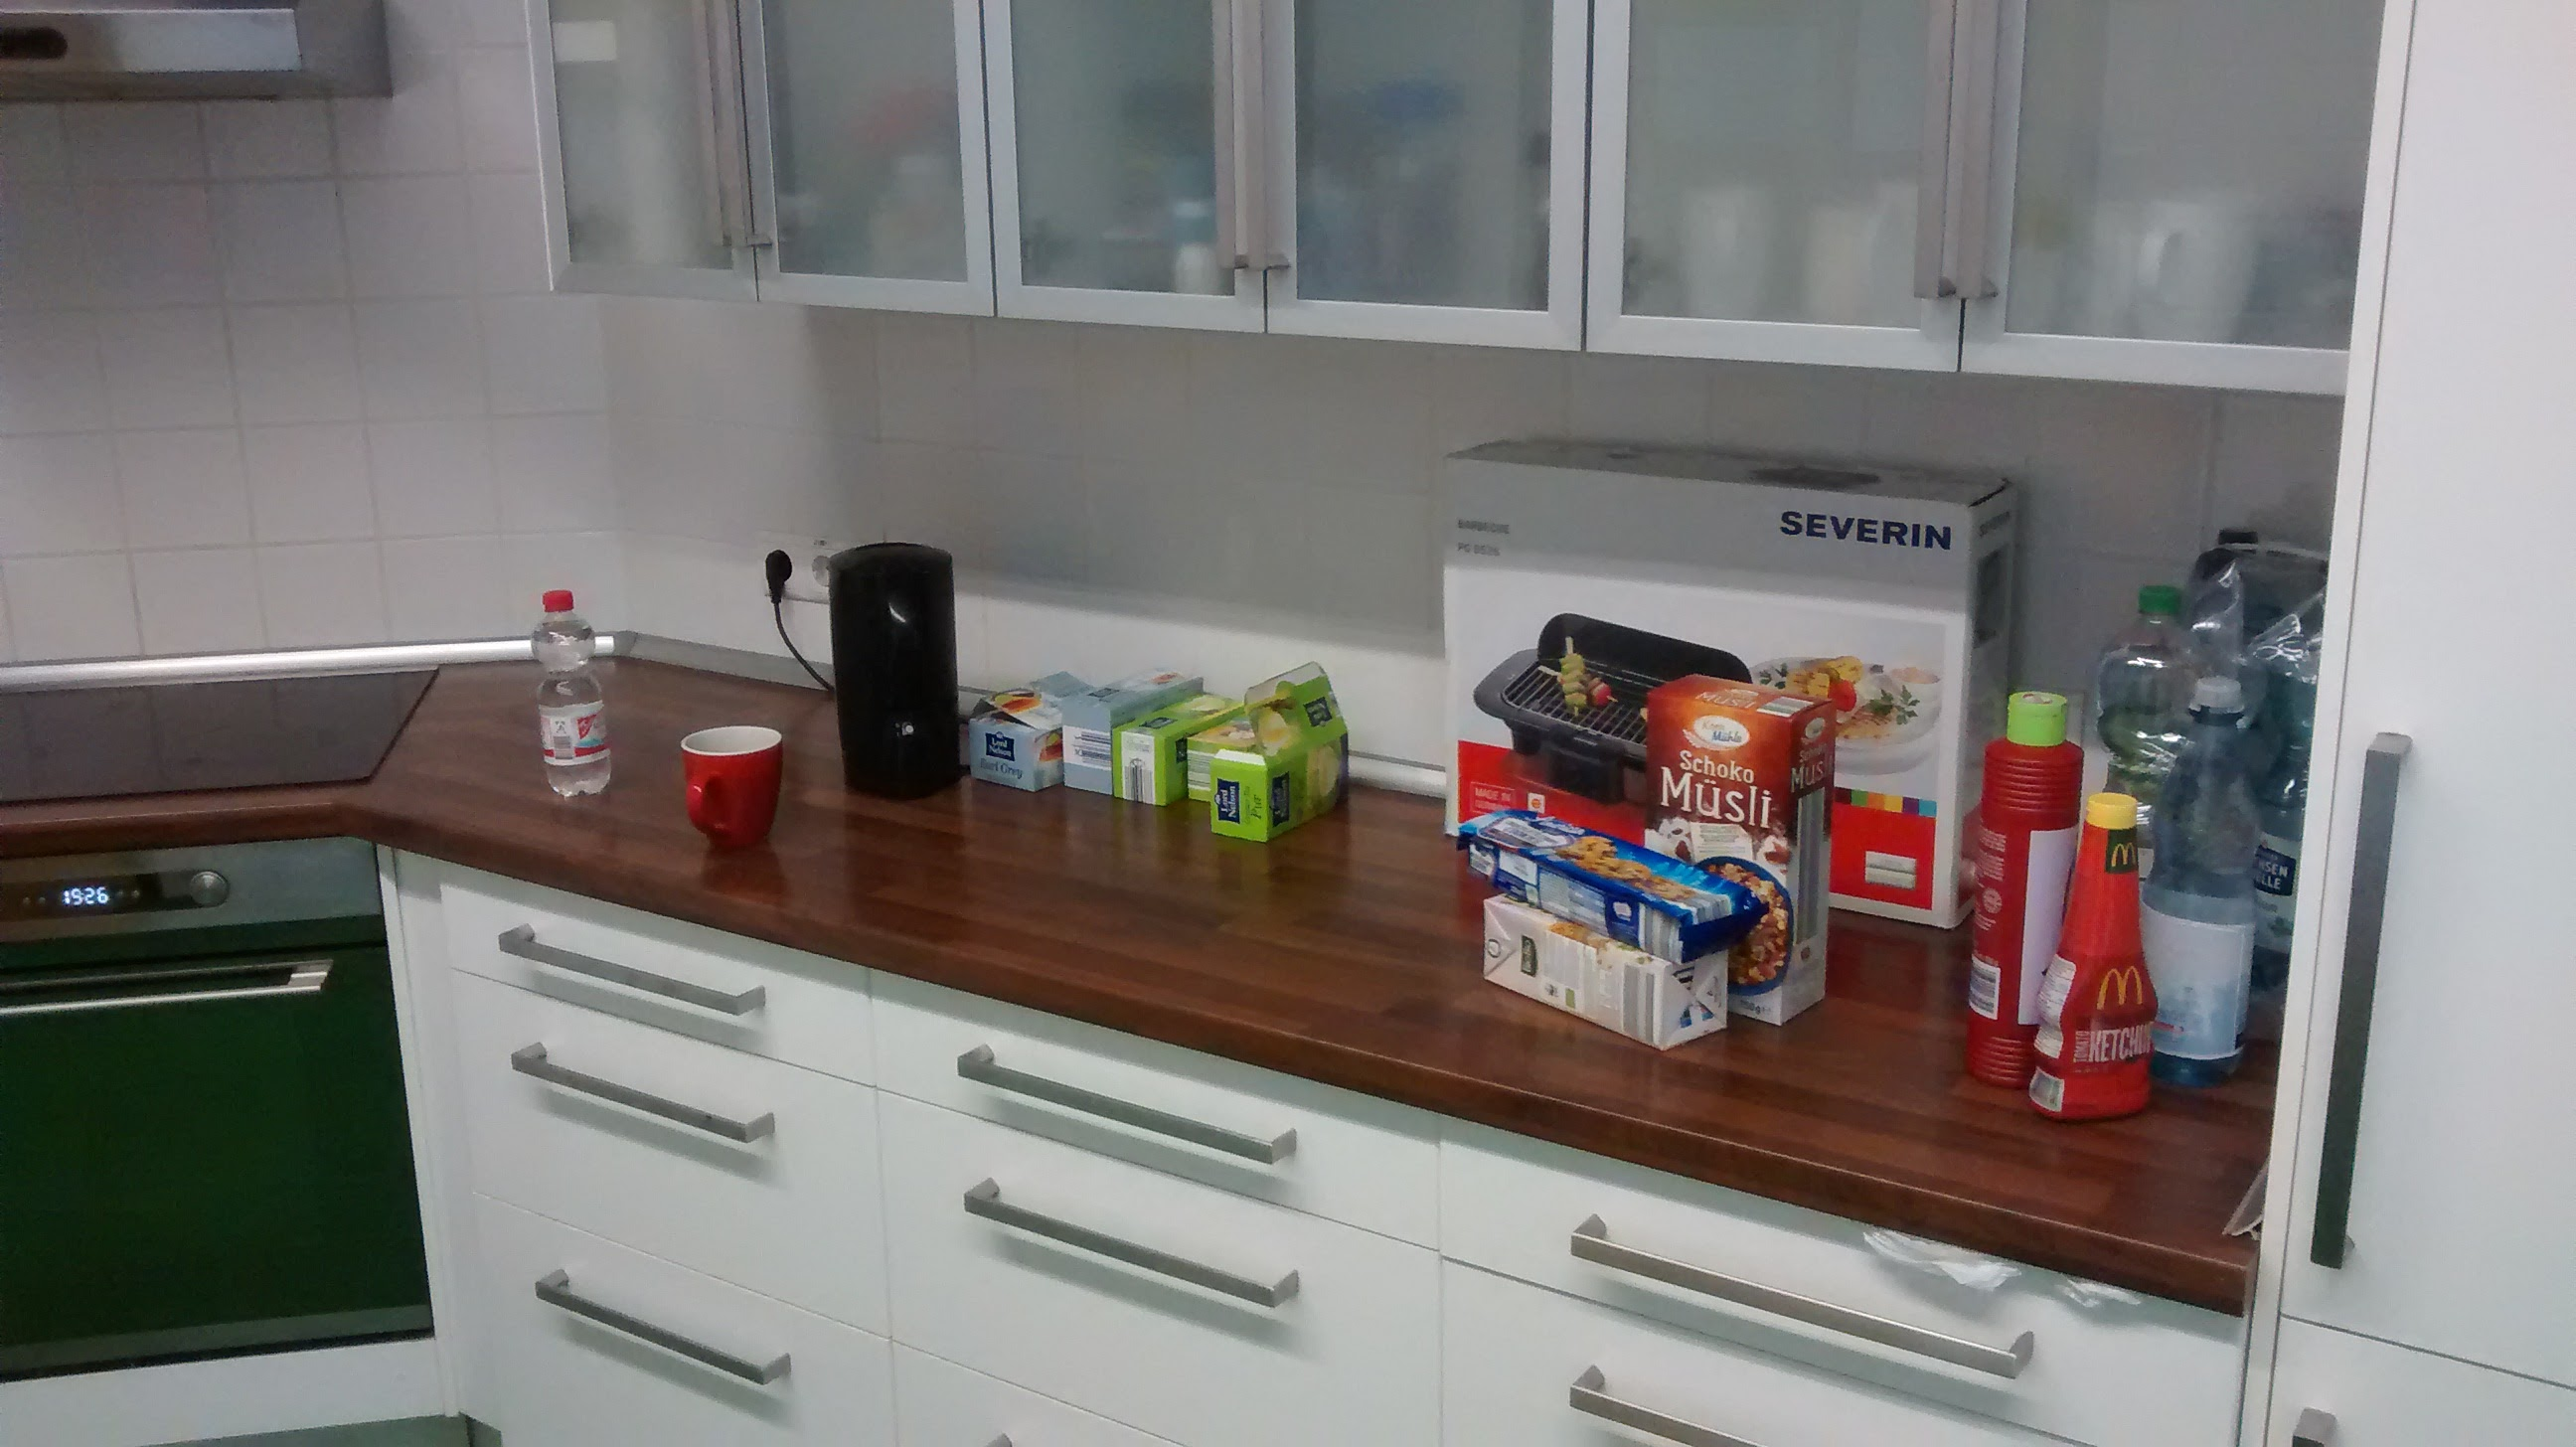
\includegraphics[width=\textwidth]{images/counter-top.jpg}
        \caption{counter-top}
        \label{fig:counter-top}
    \end{subfigure}
    \caption{Different possible object locations}\label{fig:alllocations}
\end{figure}


Thus models are developed which on absence of information of an object at a particular location decreases the probability of finding the object at that particular location while increasing the probabilities for other locations.


\FloatBarrier
\section{Hierarchical Dirichlet Categorical Bernoulli Model}

Hierarchical Dirichlet Categorical Bernoulli model (HDCB) is formed by combining the Dirichlet Categorical model and Bernoulli distribution.
For incorporating the absence observations we extended the Hierarchical Dirichlet Categorical model  with a Bernoulli distribution.
In chapter \ref{chapter: object} patterns in a single location were learned using a Beta Bernoulli model, in chapter \ref{chapter:Human location} we introduced the Dirichlet Categorical model which could reason about multiple locations in single model, here we combine both the models. The Beta Bernoulli model has the capability to learn from both success and failure results, this capability is added to the Dirichlet-Categorical model using a mixture node. 

The Bernoulli-trick is one way of making negative observations for certain location reduce its chances while making equally likely for the other locations. Thus, the location on which the object is not found are filtered out as impossible and the others are equally likely. The graphical diagram of the model is explained in \ref{dcbm}

The model is an extension as explained in \ref{sec: HDCM} . We combine a Bernoulli node $\gamma$ with the categorical node $x$. The Bernoulli is also an observation node as the categorical node. The observations are fed to the model to both the Bernoulli node and the categorical node. Suppose there are 3 locations where a object can be located. For a positive observation of locating the object at a location we feed [1.0 , 0.0, 0.0] to the Bernoulli node, where 1.0 represents object found at at location. For a negative observation i.e. the object not being found at a location the Bernoulli is given [0.0, 0.5, 0.5], where 0.0 signifies that no data was observed whereas the 0.5 increases uniformly the chances in the other locations.


\noindent
\begin{figure}[htp]
\qquad
\begin{minipage}{0.3\textwidth}
\centering

\tikz {
\node [const]                   (alpha) {$\alpha$};
\node [below=of alpha, latent]  (beta)  {$\beta$};
\node [below=of beta, latent]   (theta) {$\theta_i$};
\node [below=of theta, obs]     (x)     {$x_{ij}$};
\node [right=of x , xshift=0.05cm, obs]      (gamma) {$\gamma_{ij}$};
\edge {alpha} {beta};
\edge {beta} {theta};
\edge {theta} {x};
\edge {gamma} {x};
\plate {trials} {(x)(gamma)} {j location};
\plate {bags} {(theta)(x)(gamma)(trials)} {i time};
}

\end{minipage}%
\begin{minipage}{0.7\textwidth}

\begin{equation*}
	\alpha = <1, 1, .... , 1 > 
\end{equation*}
\begin{equation*}
	\beta \sim Dirichlet(\alpha)
\end{equation*}
\begin{equation*}
	\theta_i  \sim Dirichlet(\beta)
\end{equation*}
\begin{equation*}
	\gamma_{ij}  \sim Bernoulli(k)
\end{equation*}
\begin{equation*}
	x_{ij} \sim Categorical(\theta_i)
\end{equation*}
\end{minipage}

\caption[Dirichlet Categorical Bernoulli graphical model]{Graphical model representation of Dirichlet Categorical Bernoulli model. The boxes are ``plates" representing replicates. The outer plates represents hours of a day, while the inner plate represents if object was observed at the location each hour.}
\label{dcbm}
\end{figure}



\section{Experiments}

In this section, we present the results of a thorough evaluation of all aspects of our proposed model. We present a detailed analysis of our model on synthetic data. In particular, we study the performance of the model as compared to the HDC model discussed in chapter ~\ref{chapter:Human location}.


The goal of the experiments was to comparatively evaluate the proposed method with the HDC model, based on the number of experiments. For this we created a simulated dataset with known ground truth distributions. The observations were then by the models to learn the latent probabilities. The learned probabilities were then compared with the ground truth. 

\subsection{Simulated Dataset: Occluded Kitchen Object Dataset}

To demonstrate the proposed approach we generate a kitchen object dataset. The dataset is an extension of the dataset as developed in chapter~\ref{chapter:Human location}. To incorporate the occlusion information we generate both the presence and absence information of each object. The dataset consist of the observations of an object, cup in the home environment. The robot can scan 4 locations in the kitchen: sink, counter-top, stove and cabinet. The time of the scan is discretized into 3 times of the day: morning, afternoon and night. 

The generative process for each possible observation(present and absent) in the dataset 
\begin{itemize}
    \item Choose $ \theta \sim Dirichlet(\alpha)$ (Distribution of object over location-time)
    \item Choose randomly the time period $i$.
	\item Choose the location $x_n$ $\sim$ Categorical$(\theta_i)$
	\item Choose the presence of object $p_n$, in time period $i$ and location $x_n$  $p_n$ $\sim$ Bernoulli$(\beta) $
\end{itemize}

Ground truth of the distribution in the object location distribution over time in shown in Figure \ref{absent-gt}. The figure represents the hinton plot of the underlying Dirichlet distributions. In the ground truth probability in Figure \ref{absent-gt} the each row represents the distribution of the object cup at the particular time period. We see a big white box at location:sink and time:night on the bottom left of the plot, while all other boxes for row night are comparatively small. This signifies that the box is more likely to be found in the sink in the night than the other places.


\begin{figure}[htp]
\centering
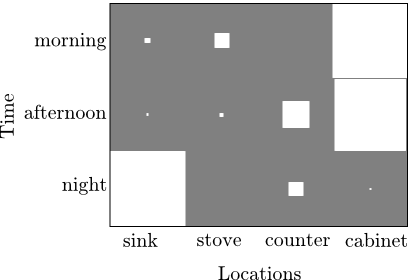
\includegraphics[width=0.6\textwidth]{images/absent_groundtruth.png}
\caption[Simulated object location ground truth distribution]{Simulated object location ground truth distribution.
The x-axis represents the locations the y axis represents the timezones. The size of the white box indicates the probability of the object presence.}
\label{absent-gt}
\end{figure}

From the ground truth we can observe that there is higher probability to find the object in the sink during night time and in the cabinet during the other time periods. We evaluate our models on these synthetic observations. 

\section{Posterior Probability Check}
The first method was to visually compare the posterior probabilities with the ground truth.  Figure~\ref{fig:absent-eval} we can visually analyse the difference between the learned models of both HDC model and HDCB model. The leftmost plot \ref{fig:absent-gt} as explained above is the ground truth from which the observations were generated. We generated a dataset with 100 observations. Out of the 100 observations 33 were positive samples while remaining were 77 were negative samples. Thus the dataset had more absent information than presence of the object. The models learned from the generated dataset. The middle plot \ref{fig:absent-hdcm} is the learned posterior probabilities using the HDC model while the last plot \ref{fig:absent-hdcmb} is the posterior probabilities using the HDCB model presented in this chapter. We can conclude from the plots that the posterior of the HDCB model resembles more with the ground truth probability. 

\begin{figure}
    \centering
    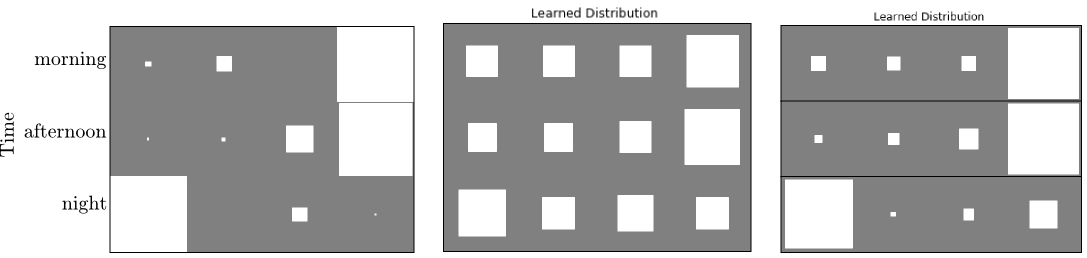
\includegraphics[width=\textwidth]{images/absent_learned.png}
       
    \begin{minipage}[t]{.35\textwidth}
    %\centering
    \subcaption{Ground Truth}\label{fig:absent-gt}
    \end{minipage}%
    \begin{minipage}[t]{.3\textwidth}
    %\centering
    \subcaption{HDC model}\label{fig:absent-hdcm}
    \end{minipage}
    \begin{minipage}[t]{.25\textwidth}
    %\centering
    \subcaption{HDCB model}\label{fig:absent-hdcmb}
    \end{minipage}

\caption[Posterior probabilities of HDC and HDCB ]{Posterior probabilities of the models : \ref{fig:absent-gt} is ground truth of the distribution. \ref{fig:absent-hdcm} is the learned distribution using the HDC model. \ref{fig:absent-hdcmb} is the learned distribution using the HDCB  model . The x-axis represents the locations the y axis represents the timezones. The size of the white box indicates the probability of the object presence }\label{fig:absent-eval}
    
\end{figure}


\section{Model Comparison}

We now quantitatively compare the Dirichlet Categorical Bernoulli model with the Hierarchical Dirichlet Categorical model. We adopted  the Bhattacharyya distance \cite{bhattacharyya1946measure} and Kullback–Leibler divergence \cite{kullback1951information} to quantify the similarity between the simulated and the learned Dirichlet  distribution. 
We generated dataset with increasing number of observations from 30 to 1000. For each sample set we trained both the models and their corresponding distance with the ground truth were recorded. The process was repeated 1000 times for each sample set.



\begin{figure}[htp]
\centering

\begin{subfigure}{.45\textwidth}
  \centering
  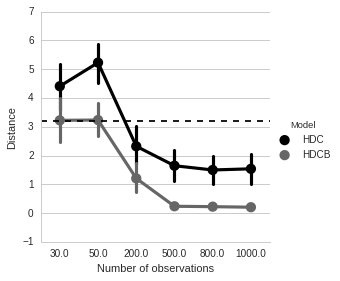
\includegraphics[width=\linewidth]{images/HDCB-Bhattacharya-Distance.png}
    \caption{Bhattacharyya distance}
\end{subfigure}
\begin{subfigure}{.45\textwidth}
  \centering
  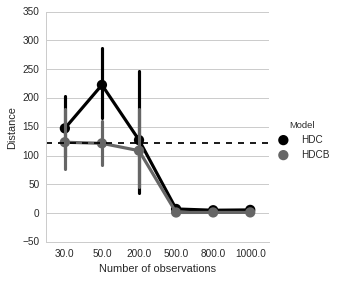
\includegraphics[width=\linewidth]{images/HDCB-KL-Distance.png}
    \caption{Kullback–Leibler divergence}
\end{subfigure}

\caption[Model evaluation]{Measure of the distance between the learned probabilities and ground truth for models HDC and HDCB. The x-axis represents the different sample size.}
\label{fig:B-KL-evaluation}
\end{figure}

Figure~\ref{fig:B-KL-evaluation} comparatively plots the distance with the ground truth with different sample set. As expected with increasing number of sample set the distance between the learned and the ground truth reduces after 500 observations the learning is almost stable and saturated. Also the spread of the results is decreasing with increasing number of samples, thus indicating the model is getting more confident on its learning. 

From the Figure~\ref{fig:B-KL-evaluation} we observe that for 30 observations the Bhattacharyya distance  and KL divergence for the HDCB model is 3 and 125 respectively. While for the HDC model is quite high around 4.5 and 150 respectively. For the HDC model to reduce its distance around to the 3/125 it needs to have a dataset with more than 100 observations, this is shown by the dashed line in the figure. From this we can experiments we can conclusively conclude the HDCB model can learn with less observations as compared to HDC model.
 

\section{Discussions}

In this chapter, we presented a Bayesian probabilistic model for learning user preferences in object placement in highly occluded environments like home. We include the information of the absence of the object at particular location to increase the probability of other locations. In extensive experiments carried out using simulated dataset, we demonstrated that the proposed model learns with lesser number of demonstrations as compared to the model which only learns from presence of object observations. Our model combines the features of Beta-Bernoulli and Dirichlet-Categorical models. Our approach enables domestic service robots to learn about user preferences about object location home environments more robustly.